\documentclass{minimal}

\usepackage{tikz}
\usepackage{tikz-3dplot}
\usepackage{circuitikz}
\usepackage{graphicx}
\usepackage{color}
\usepackage[absolute,overlay]{textpos}
  \setlength{\TPHorizModule}{1mm}
  \setlength{\TPVertModule}{1mm}
\usepackage{xcolor}
\usepackage{calc}
\usepackage{amssymb}
  
\usepackage{tikz}
\usepackage{steinmetz}
\usepackage{color}
\usepackage{tcolorbox}
\usetikzlibrary{shapes.geometric, arrows}
\usepackage{rotating}
\usepackage{pgfplots}
\usepackage{url}

\usetikzlibrary{shapes,snakes}
\usetikzlibrary{patterns}


\usetikzlibrary{arrows,shapes,positioning}
\usetikzlibrary{calc,decorations.markings}

\begin{document}

\newcommand{\ve}[1]{\ensuremath{\mathbf{#1}}}
\newcommand{\ud}[0]{\mathrm{d}}

\tikzset{
    vector/.style = {
        thick,
        > = stealth',
    },
    axis/.style = {
        very thin,
        > = stealth',
    },
}


\tdplotsetmaincoords{70}{100}
\tdplotsetrotatedcoords{90}{90}{90}
\begin{tikzpicture}[tdplot_main_coords]
%\begin{tikzpicture}
    \draw (0,0,0) -- ++(0,-2.3,0);
    
    \draw (0,0) to (0,-3) node[ground]{};

    % draw a condensor plate
    \draw[fill=lightgray] (-1.5,0,-1.5)--(-1.5,0,1.5)--(1.5,0,1.5)--(1.5,0,-1.5)--cycle;
    \draw[fill=lightgray] (1.5,0,-1.5)--(1.5,-0.2,-1.5)--(1.5,-0.2,1.5)--(1.5,0,1.5)--cycle;
    \draw[fill=lightgray] (1.5,-0.2,1.5)--(-1.5,-0.2,1.5)--(-1.5,0,1.5)--(1.5,0,1.5)--cycle;

    \def\q{-5.3}
    
    
    \draw[<-,color=red] (1,0,1)--++(0,-\q,0);
    \draw[<-,color=red] (-1,0,1)--++(0,-\q,0);
    
    \draw[<-,color=red] (1,0,-1)--++(0,-\q,0);
    \draw[<-,color=red] (-1,0,-1)--++(0,-\q,0);
    
    % draw second condensor plate
    \draw[fill=lightgray] (-1.5,0-\q,-1.5)--(-1.5,0-\q,1.5)--(1.5,0-\q,1.5)--(1.5,0-\q,-1.5)--cycle;
    \draw[fill=lightgray] (1.5,0-\q,-1.5)--(1.5,-0.2-\q,-1.5)--(1.5,-0.2-\q,1.5)--(1.5,0-\q,1.5)--cycle;
    \draw[fill=lightgray] (1.5,-0.2-\q,1.5)--(-1.5,-0.2-\q,1.5)--(-1.5,0-\q,1.5)--(1.5,0-\q,1.5)--cycle;
    
    \draw (0,-\q,0)--++(0,2,0)node[above right]{$+$};
    
\end{tikzpicture}%


\newpage


\tdplotsetmaincoords{70}{100}
\tdplotsetrotatedcoords{90}{90}{90}
\begin{tikzpicture}[tdplot_main_coords]
%\begin{tikzpicture}
	\def\q{-2.3}
    \draw (0,0,0) -- ++(0,\q,0);
    
    \draw (0,0) to (0,-3) node[ground]{};
    
    \draw[->,color=blue!50,style=thick] (-1,-2) to (-1,-4)  to (-1, -4,-0.5) node[above left]{$I$};

    % draw a condensor plate
    \draw[fill=lightgray] (-1.5,0,-1.5)--(-1.5,0,1.5)--(1.5,0,1.5)--(1.5,0,-1.5)--cycle;
    \draw[fill=lightgray] (1.5,0,-1.5)--(1.5,-0.2,-1.5)--(1.5,-0.2,1.5)--(1.5,0,1.5)--cycle;
    \draw[fill=lightgray] (1.5,-0.2,1.5)--(-1.5,-0.2,1.5)--(-1.5,0,1.5)--(1.5,0,1.5)--cycle;
    
    \draw[<-,color=red] (0,0,0)--++(0,-\q,0);
    \draw[<-,color=red] (1,0,0)--++(0,-\q,0);
    \draw[<-,color=red] (-1,0,0)--++(0,-\q,0);
    
    \draw[<-,color=red] (0,0,1)--++(0,-\q,0);
    \draw[<-,color=red] (1,0,1)--++(0,-\q,0);
    \draw[<-,color=red] (-1,0,1)--++(0,-\q,0);
    
    \draw[<-,color=red] (0,0,-1)--++(0,-\q,0);
    \draw[<-,color=red] (1,0,-1)--++(0,-\q,0);
    \draw[<-,color=red] (-1,0,-1)--++(0,-\q,0);

    % draw second condensor plate
    \draw[fill=lightgray] (-1.5,0-\q,-1.5)--(-1.5,0-\q,1.5)--(1.5,0-\q,1.5)--(1.5,0-\q,-1.5)--cycle;
    \draw[fill=lightgray] (1.5,0-\q,-1.5)--(1.5,-0.2-\q,-1.5)--(1.5,-0.2-\q,1.5)--(1.5,0-\q,1.5)--cycle;
    \draw[fill=lightgray] (1.5,-0.2-\q,1.5)--(-1.5,-0.2-\q,1.5)--(-1.5,0-\q,1.5)--(1.5,0-\q,1.5)--cycle;
    
    \draw (0,-\q,0)--++(0,2,0)node[above right]{$+$};
    
    
\end{tikzpicture}%


\newpage


\tdplotsetmaincoords{70}{100}
\tdplotsetrotatedcoords{90}{90}{90}
\begin{tikzpicture}[tdplot_main_coords]
%\begin{tikzpicture}
	\def\q{-2.3}
    \draw (0,0,0) -- ++(0,\q,0);
    
    \draw (0,0) to (0,\q) node[ground]{};

    % draw a condensor plate
    \draw[fill=lightgray] (-1.5,0,-1.5)--(-1.5,0,1.5)--(1.5,0,1.5)--(1.5,0,-1.5)--cycle;
    \draw[fill=lightgray] (1.5,0,-1.5)--(1.5,-0.2,-1.5)--(1.5,-0.2,1.5)--(1.5,0,1.5)--cycle;
    \draw[fill=lightgray] (1.5,-0.2,1.5)--(-1.5,-0.2,1.5)--(-1.5,0,1.5)--(1.5,0,1.5)--cycle;
    
    
    % dielectric
    \draw[fill=blue!20,opacity=0.8] (-1.5,-\q,1.5)--(-1.5,0,1.5)--(1.5,0,1.5)--(1.5,-\q,1.5)--cycle;
    \draw[fill=blue!20,opacity=0.8] (1.5,-\q,1.5)--(1.5,0,1.5)--(1.5,0,-1.5)--(1.5,-\q,-1.5)--cycle;
    %\draw[fill=blue!20] (1.5,0-\q,-1.5)--(1.5,\q,-1.5)--(1.5,\q,1.5)--(1.5,0-\q,1.5)--cycle;
    %\draw[fill=blue!20] (1.5,-0.2-\q,1.5)--(-1.5,-0.2-\q,1.5)--(-1.5,0-\q,1.5)--(1.5,0-\q,1.5)--cycle;
    
    
    
    
    %\draw[<-,color=red] (0,0,0)--++(0,-\q,0);
    %\draw[<-,color=red] (1,0,0)--++(0,-\q,0);
    %\draw[<-,color=red] (-1,0,0)--++(0,-\q,0);
    
    %\draw[<-,color=red] (0,0,1)--++(0,-\q,0);
    %\draw[<-,color=red] (1,0,1)--++(0,-\q,0);
    %\draw[<-,color=red] (-1,0,1)--++(0,-\q,0);
    
    %\draw[<-,color=red] (0,0,-1)--++(0,-\q,0);
    %\draw[<-,color=red] (1,0,-1)--++(0,-\q,0);
    %\draw[<-,color=red] (-1,0,-1)--++(0,-\q,0);

    % draw second condensor plate
    \draw[fill=lightgray] (-1.5,0-\q,-1.5)--(-1.5,0-\q,1.5)--(1.5,0-\q,1.5)--(1.5,0-\q,-1.5)--cycle;
    \draw[fill=lightgray] (1.5,0-\q,-1.5)--(1.5,-0.2-\q,-1.5)--(1.5,-0.2-\q,1.5)--(1.5,0-\q,1.5)--cycle;
    \draw[fill=lightgray] (1.5,-0.2-\q,1.5)--(-1.5,-0.2-\q,1.5)--(-1.5,0-\q,1.5)--(1.5,0-\q,1.5)--cycle;
    
    \draw (0,-\q,0)--++(0,2,0);
    
    
\end{tikzpicture}%

\newpage


\tdplotsetmaincoords{70}{100}
\tdplotsetrotatedcoords{90}{90}{90}
\begin{tikzpicture}[tdplot_main_coords]
%\begin{tikzpicture}
	\def\q{-2.3}
    \draw (0,0,0) -- ++(0,\q,0);
    
    \draw (0,0) to (0,\q) node[ground]{};

    % draw a condensor plate
    \draw[fill=lightgray] (-1.5,0,-1.5)--(-1.5,0,1.5)--(1.5,0,1.5)--(1.5,0,-1.5)--cycle;
    \draw[fill=lightgray] (1.5,0,-1.5)--(1.5,-0.2,-1.5)--(1.5,-0.2,1.5)--(1.5,0,1.5)--cycle;
    \draw[fill=lightgray] (1.5,-0.2,1.5)--(-1.5,-0.2,1.5)--(-1.5,0,1.5)--(1.5,0,1.5)--cycle;
    
    
    % dielectric
    \draw[fill=blue!20,opacity=0.8] (-1.5,-\q,1.5)--(-1.5,0,1.5)--(1.5,0,1.5)--(1.5,-\q,1.5)--cycle;
    \draw[fill=blue!20,opacity=0.8] (1.5,-\q,1.5)--(1.5,0,1.5)--(1.5,0,-1.5)--(1.5,-\q,-1.5)--cycle;
    %\draw[fill=blue!20] (1.5,0-\q,-1.5)--(1.5,\q,-1.5)--(1.5,\q,1.5)--(1.5,0-\q,1.5)--cycle;
    %\draw[fill=blue!20] (1.5,-0.2-\q,1.5)--(-1.5,-0.2-\q,1.5)--(-1.5,0-\q,1.5)--(1.5,0-\q,1.5)--cycle;
    
    
    
    
    %\draw[<-,color=red] (0,0,0)--++(0,-\q,0);
    %\draw[<-,color=red] (1,0,0)--++(0,-\q,0);
    %\draw[<-,color=red] (-1,0,0)--++(0,-\q,0);
    
    %\draw[<-,color=red] (0,0,1)--++(0,-\q,0);
    %\draw[<-,color=red] (1,0,1)--++(0,-\q,0);
    %\draw[<-,color=red] (-1,0,1)--++(0,-\q,0);
    
    %\draw[<-,color=red] (0,0,-1)--++(0,-\q,0);
    %\draw[<-,color=red] (1,0,-1)--++(0,-\q,0);
    %\draw[<-,color=red] (-1,0,-1)--++(0,-\q,0);

    % draw second condensor plate
    \draw[fill=lightgray] (-1.5,0-\q,-1.5)--(-1.5,0-\q,1.5)--(1.5,0-\q,1.5)--(1.5,0-\q,-1.5)--cycle;
    \draw[fill=lightgray] (1.5,0-\q,-1.5)--(1.5,-0.2-\q,-1.5)--(1.5,-0.2-\q,1.5)--(1.5,0-\q,1.5)--cycle;
    \draw[fill=lightgray] (1.5,-0.2-\q,1.5)--(-1.5,-0.2-\q,1.5)--(-1.5,0-\q,1.5)--(1.5,0-\q,1.5)--cycle;
    
    \draw (0,-\q,0)--++(0,2,0);
    
    
    \begin{scope}[canvas is yz plane at x=0]
     \draw[fill=blue!30] (-\q/2-0.3,0) circle (0.2);
     \draw[style=thick] (-\q/2-0.5,0) to (0,-3);
     \draw[style=thick] (-\q/2-0.1,0) to (-\q,-3);
     
     \def\d{3};
     \draw[fill=blue!30] (-\q/2,-\q-3-\d) circle (\d/2) node{\color{red}\textbf{+}};
     
     \tikzset{shift={(-\q/2,-\q-3-\d)}}
     %\foreach \a in {1,2,...,8}{
     %\draw (\a*360/8: \d/2.5) node{$\color{blue} -$};
     %}
   \end{scope}
	
\end{tikzpicture}


\vspace{1cm}


\tdplotsetmaincoords{70}{100}
\tdplotsetrotatedcoords{90}{90}{90}
\begin{tikzpicture}[tdplot_main_coords]
%\begin{tikzpicture}
	\def\q{-2.3}
    \draw (0,0,0) -- ++(0,\q,0);
    
    \draw (0,0) to (0,\q) node[ground]{};

    % draw a condensor plate
    \draw[fill=lightgray] (-1.5,0,-1.5)--(-1.5,0,1.5)--(1.5,0,1.5)--(1.5,0,-1.5)--cycle;
    \draw[fill=lightgray] (1.5,0,-1.5)--(1.5,-0.2,-1.5)--(1.5,-0.2,1.5)--(1.5,0,1.5)--cycle;
    \draw[fill=lightgray] (1.5,-0.2,1.5)--(-1.5,-0.2,1.5)--(-1.5,0,1.5)--(1.5,0,1.5)--cycle;
    
    
    % dielectric
    \draw[fill=blue!20,opacity=0.8] (-1.5,-\q,1.5)--(-1.5,0,1.5)--(1.5,0,1.5)--(1.5,-\q,1.5)--cycle;
    \draw[fill=blue!20,opacity=0.8] (1.5,-\q,1.5)--(1.5,0,1.5)--(1.5,0,-1.5)--(1.5,-\q,-1.5)--cycle;
    %\draw[fill=blue!20] (1.5,0-\q,-1.5)--(1.5,\q,-1.5)--(1.5,\q,1.5)--(1.5,0-\q,1.5)--cycle;
    %\draw[fill=blue!20] (1.5,-0.2-\q,1.5)--(-1.5,-0.2-\q,1.5)--(-1.5,0-\q,1.5)--(1.5,0-\q,1.5)--cycle;
    
    
    
    
    %\draw[<-,color=red] (0,0,0)--++(0,-\q,0);
    %\draw[<-,color=red] (1,0,0)--++(0,-\q,0);
    %\draw[<-,color=red] (-1,0,0)--++(0,-\q,0);
    
    %\draw[<-,color=red] (0,0,1)--++(0,-\q,0);
    \draw[<-,color=red,style=thick] (1,0,1)--++(0,-\q,0);
    \draw[<-,color=red,style=thick] (-1,0,1)--++(0,-\q,0);
    
    %\draw[<-,color=red] (0,0,-1)--++(0,-\q,0);
    \draw[<-,color=red,style=thick] (1,0,-1)--++(0,-\q,0);
    \draw[<-,color=red,style=thick] (-1,0,-1)--++(0,-\q,0);

    % draw second condensor plate
    \draw[fill=lightgray] (-1.5,0-\q,-1.5)--(-1.5,0-\q,1.5)--(1.5,0-\q,1.5)--(1.5,0-\q,-1.5)--cycle;
    \draw[fill=lightgray] (1.5,0-\q,-1.5)--(1.5,-0.2-\q,-1.5)--(1.5,-0.2-\q,1.5)--(1.5,0-\q,1.5)--cycle;
    \draw[fill=lightgray] (1.5,-0.2-\q,1.5)--(-1.5,-0.2-\q,1.5)--(-1.5,0-\q,1.5)--(1.5,0-\q,1.5)--cycle;
    
    \draw (0,-\q,0)--++(0,2,0) node[above right]{+};
    
    \def\d{3};
    \begin{scope}[canvas is yz plane at x=0]
     \draw[fill=blue!30] (-\q/2-0.3,0) ellipse (\d/10 and \d/15);
     \draw[style=thick] (-\q/2-0.60,0) to (0,-3);
     \draw[style=thick] (-\q/2,0) to (-\q,-3);
     
     
     \draw[fill=blue!30] (-\q/2,-\q-3-\d) ellipse (\d/2 and \d/3) node[left]{\color{red} \textbf{+}};
     
     \tikzset{shift={(-\q/2,-\q-3-\d)}}
     \foreach \a in {1,2,...,8}{
     %\draw (\a*360/8: \d/2.5) node{$\color{blue} -$};
     }
     \draw[<-,style=thick] (0.5, -1.5) -- (-1, -1.5) node[left]{$\textbf{P}$};
   \end{scope}
	
\end{tikzpicture}


\newpage
% antennas

\tdplotsetmaincoords{70}{100}
%\tdplotsetmaincoords{0}{90}
\tdplotsetrotatedcoords{90}{90}{90}
\begin{tikzpicture}[tdplot_main_coords,scale=1]
%\begin{tikzpicture}
    \draw[style=thick] (0,-1,0) -- ++(0,-3,0);
    

	\def\o{0.0}
    % draw antenna 1
    \draw[style=thick](0,-1,0)--(1,0,0);
    \draw[style=thick](0,-1,0)--(-1,0,0);

    \def\f{-5.3}
    
	\draw[fill=blue!20,opacity=0.5] (-1.5,-\f,1.5)--(-1.5,0,1.5)--(1.5,0,1.5)--(1.5,-\f,1.5)--cycle;
    \draw[fill=blue!20,opacity=0.5] (1.5,-\f,1.5)--(1.5,0,1.5)--(1.5,0,-1.5)--(1.5,-\f,-1.5)--cycle;
    
    \draw[opacity=0.5] (-1.5,0,1.5)--(1.5,0,1.5)--(1.5,0,-1.5)--(-1.5,0,-1.5)--cycle;
    \draw[fill=blue!20,opacity=0.5] (-1.5,-\f,1.5)--(1.5,-\f,1.5)--(1.5,-\f,-1.5)--(-1.5,-\f,-1.5)--cycle;  
    
    %draw radiation lines 
    \draw[color=red] (-0.5,0.5) to [bend left=30] (0.5,0.5); 
    \draw[color=red] (-0.7,1) to [bend left=27] (0.7,1); 
    \draw[color=red] (-0.9,1.5) to [bend left=24] (0.9,1.5);
    \draw[color=red] (-1.1,2) to [bend left=21] (1.1,2);
    \draw[color=red] (-1.3,2.5) to [bend left=18] (1.3,2.5);
    \draw[color=red] (-1.5,3) to [bend left=15] (1.5,3);
    \draw[color=red] (-1.5,3.5) to [bend left=12] (1.5,3.5);
    \draw[color=red] (-1.5,4) to [bend left=9] (1.5,4);
    
    
    % draw second antenna
   \draw[style=thick](0,-\f+1,0)--(1,-\f,0);
    \draw[style=thick](0,-\f+1,0)--(-1,-\f,0);
    
    \draw[style=thick](0,-\f+1,0)--(0,-\f+3,0);
    
\end{tikzpicture}%


\newpage


\tdplotsetmaincoords{70}{120}
\tdplotsetrotatedcoords{90}{90}{90}
\begin{tikzpicture}[tdplot_main_coords,scale=0.5]
	\draw[fill=lightgray] (-2,-2)--(-2,2)--(2,2)--(2,-2)--(-2,-2);
	\draw[fill=lightgray] (2,-2,0)--(2,2,0)--(2,2,-4)--(2,-2,-4)--(2,-2,0);\
	\draw (2,0,-2) circle (1);
\end{tikzpicture}


\newpage


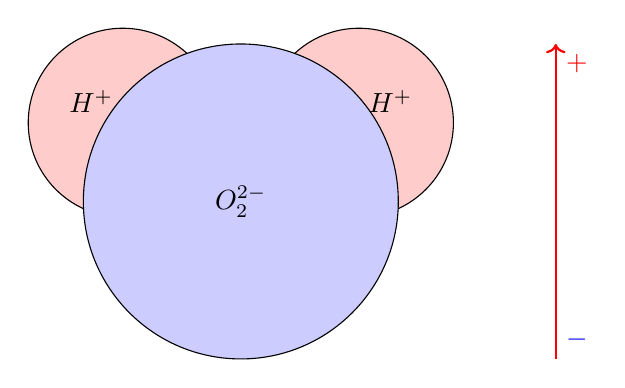
\begin{tikzpicture}
	\draw[fill=red!20] (1.5,1) circle (1.2) node [above right] {$H^+$};
	\draw[fill=red!20] (-1.5,1) circle (1.2) node [above left] {$H^+$};
	\draw[fill=blue!20] (0,0) circle (2) node {$O_2^{2-}$};
	
	\draw[<-, color=red, style=thick] (4,2) node[below right]{$\color{red}+$} to (4,-2) node[above right]{$\color{blue}-$};
\end{tikzpicture}


\newpage


\tdplotsetmaincoords{70}{100}
\tdplotsetrotatedcoords{90}{90}{90}
\begin{tikzpicture}[tdplot_main_coords]
%\begin{tikzpicture}
	\def\q{-2.3}
    \draw (0,0,0) -- ++(0,\q,0);
    
    \draw (0,0) to (0,\q) node[ground]{};

    % draw a condensor plate
    \draw[fill=lightgray] (-1.5,0,-1.5)--(-1.5,0,1.5)--(1.5,0,1.5)--(1.5,0,-1.5)--cycle;
    \draw[fill=lightgray] (1.5,0,-1.5)--(1.5,-0.2,-1.5)--(1.5,-0.2,1.5)--(1.5,0,1.5)--cycle;
    \draw[fill=lightgray] (1.5,-0.2,1.5)--(-1.5,-0.2,1.5)--(-1.5,0,1.5)--(1.5,0,1.5)--cycle;
    
    
    % dielectric
    \draw[fill=blue!20,opacity=0.7] (-1.5,-\q,1.5)--(-1.5,0,1.5)--(1.5,0,1.5)--(1.5,-\q,1.5)--cycle;
    \draw[fill=blue!20,opacity=0.7] (1.5,-\q,1.5)--(1.5,0,1.5)--(1.5,0,-1.5)--(1.5,-\q,-1.5)--cycle;
    %\draw[fill=blue!20] (1.5,0-\q,-1.5)--(1.5,\q,-1.5)--(1.5,\q,1.5)--(1.5,0-\q,1.5)--cycle;
    %\draw[fill=blue!20] (1.5,-0.2-\q,1.5)--(-1.5,-0.2-\q,1.5)--(-1.5,0-\q,1.5)--(1.5,0-\q,1.5)--cycle;
    
    \draw[<-,color=red,style=thick] (1,0,1) to (1,-\q,1);
    \draw[<-,color=red,style=thick] (1,0,-1) to (1,-\q,-1);
    \draw[<-,color=red,style=thick] (-1,0,1) to (-1,-\q,1);
    \draw[<-,color=red,style=thick] (-1,0,-1) to (-1,-\q,-1);
    
    \draw[->,style=thick] (1,0.8,0) to (1,-\q-0.8,0);
    \draw[->,style=thick] (-1,0.8,0) to (-1,-\q-0.8,0);
    
    
    %\draw[<-,color=red] (0,0,0)--++(0,-\q,0);
    %\draw[<-,color=red] (1,0,0)--++(0,-\q,0);
    %\draw[<-,color=red] (-1,0,0)--++(0,-\q,0);
    
    %\draw[<-,color=red] (0,0,1)--++(0,-\q,0);
    %\draw[<-,color=red] (1,0,1)--++(0,-\q,0);
    %\draw[<-,color=red] (-1,0,1)--++(0,-\q,0);
    
    %\draw[<-,color=red] (0,0,-1)--++(0,-\q,0);
    %\draw[<-,color=red] (1,0,-1)--++(0,-\q,0);
    %\draw[<-,color=red] (-1,0,-1)--++(0,-\q,0);

    % draw second condensor plate
    \draw[fill=lightgray] (-1.5,0-\q,-1.5)--(-1.5,0-\q,1.5)--(1.5,0-\q,1.5)--(1.5,0-\q,-1.5)--cycle;
    \draw[fill=lightgray] (1.5,0-\q,-1.5)--(1.5,-0.2-\q,-1.5)--(1.5,-0.2-\q,1.5)--(1.5,0-\q,1.5)--cycle;
    \draw[fill=lightgray] (1.5,-0.2-\q,1.5)--(-1.5,-0.2-\q,1.5)--(-1.5,0-\q,1.5)--(1.5,0-\q,1.5)--cycle;
    
    \draw (0,-\q,0)--++(0,2,0)node[above right]{$+$};
    
    
\end{tikzpicture}%




\newpage


\tdplotsetmaincoords{80}{100}
\tdplotsetrotatedcoords{90}{90}{90}
\begin{tikzpicture}[tdplot_main_coords]
%\begin{tikzpicture}
	\def\q{-3};
	\def\h{4}
	
	\draw[->,color=red, style=thick] (0,-\q/2,1.5) .. controls(0,-\q/2+0.5,0.5) .. (0,-\q/2+1,1.5);
	\draw[->,color=red, style=thick] (0,-\q/2,1.5) .. controls(0,-\q/2-0.5,0.5) .. (0,-\q/2-1,1.5);
    
    
    % dielectric
    \draw[fill=blue!20,opacity=0.5] (-1.5,-\q,1.5)--(-1.5,0,1.5)--(1.5,0,1.5)--(1.5,-\q,1.5)--cycle;
    \draw[fill=blue!20,opacity=0.5] (1.5,-\q,1.5)--(1.5,0,1.5)--(1.5,0,-1.5)--(1.5,-\q,-1.5)--cycle;
    \draw[fill=blue!20,opacity=0.5] (1.5,-\q,-1.5)--(1.5,-\q,1.5)--(-1.5,-\q,1.5)--(-1.5,-\q,-1.5)--cycle;
    %\draw[fill=blue!20] (1.5,-0.2-\q,1.5)--(-1.5,-0.2-\q,1.5)--(-1.5,0-\q,1.5)--(1.5,0-\q,1.5)--cycle;
    
    
    %\draw (0,-\q/2-1,1.5)--(0,-\q/2+1,1.5)--(0,-\q/2+1,\h)--(0,-\q/2-1,\h)--(0,-\q/2-1,1.5);  
	\draw (0,-\q/2+1,1.5)--(0,-\q/2+1,\h); 
	\draw (0,-\q/2-1,\h)--(0,-\q/2-1,1.5);   
    \draw (0,-\q/2,1.5) circle (1);
   
	  
    \draw[fill=gray!50] (0,-\q/2,1.5) circle (0.5);
    \draw[fill=gray!50] (0,-\q/2+0.5,1.5)--(0,-\q/2+0.5,\h)--(0,-\q/2-0.5,\h)--(0,-\q/2-0.5,1.5);  
    \draw[fill=gray!50] (0,-\q/2,\h) circle(0.5);    
    
    \draw (0,-\q/2,\h) circle(1);
    
    
    
    
    
	
    
    % [fill=gray!20,opacity=0.6]
    
    
	
\end{tikzpicture}




\newpage

\tdplotsetmaincoords{70}{100}
\tdplotsetrotatedcoords{90}{90}{90}
\begin{tikzpicture}[tdplot_main_coords]
%\begin{tikzpicture}
	\def\q{-2.3}
    \draw (0,0,0) -- ++(0,\q,0);
    
    \draw (0,0) to (0,-3) node[ground]{};
    
    \draw[->,color=blue!50,style=thick] (-1,-2) to (-1,-4)  to (-1, -4,-0.5) node[above left]{$I$};

    % draw a condensor plate
    \draw[fill=lightgray] (-1.5,0,-1.5)--(-1.5,0,1.5)--(1.5,0,1.5)--(1.5,0,-1.5)--cycle;
    \draw[fill=lightgray] (1.5,0,-1.5)--(1.5,-0.2,-1.5)--(1.5,-0.2,1.5)--(1.5,0,1.5)--cycle;
    \draw[fill=lightgray] (1.5,-0.2,1.5)--(-1.5,-0.2,1.5)--(-1.5,0,1.5)--(1.5,0,1.5)--cycle;
    
    \draw[<-,color=red] (0,0,0)--++(0,-\q,0);
    \draw[<-,color=red] (1,0,0)--++(0,-\q,0);
    \draw[<-,color=red] (-1,0,0)--++(0,-\q,0);
    
    \draw[<-,color=red] (0,0,1)--++(0,-\q,0);
    \draw[<-,color=red] (1,0,1)--++(0,-\q,0);
    \draw[<-,color=red] (-1,0,1)--++(0,-\q,0);
    
    \draw[<-,color=red] (0,0,-1)--++(0,-\q,0);
    \draw[<-,color=red] (1,0,-1)--++(0,-\q,0);
    \draw[<-,color=red] (-1,0,-1)--++(0,-\q,0);

    % draw second condensor plate
    \draw[fill=lightgray] (-1.5,0-\q,-1.5)--(-1.5,0-\q,1.5)--(1.5,0-\q,1.5)--(1.5,0-\q,-1.5)--cycle;
    \draw[fill=lightgray] (1.5,0-\q,-1.5)--(1.5,-0.2-\q,-1.5)--(1.5,-0.2-\q,1.5)--(1.5,0-\q,1.5)--cycle;
    \draw[fill=lightgray] (1.5,-0.2-\q,1.5)--(-1.5,-0.2-\q,1.5)--(-1.5,0-\q,1.5)--(1.5,0-\q,1.5)--cycle;
    
    \draw (0,-\q,0)--++(0,2,0)node[above right]{$+$};
    
    
\end{tikzpicture}%




\newpage


\tdplotsetrotatedcoords{90}{90}{90}
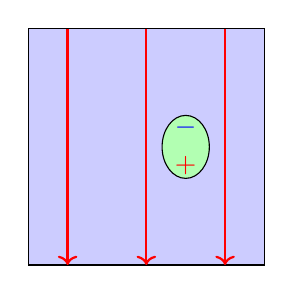
\begin{tikzpicture}
	\draw[fill=blue!20] (-1.5,-1.5)--(-1.5,1.5)--(1.5,1.5)--(1.5,-1.5)--(-1.5,-1.5);
	
	\draw[->,color=red,style=thick] (1,1.5)--(1,-1.5);
	\draw[->,color=red,style=thick] (-1,1.5)--(-1,-1.5);
	\draw[->,color=red,style=thick] (0,1.5)--(0,-1.5);
	
	\draw[fill=green!30] (0.5,0) ellipse (0.3 and 0.4) node[below]{$\color{red}+$} node[above]{$\color{blue}-$};
	
\end{tikzpicture}



\newpage

\tikzset{%
  every neuron/.style={
    circle,
    draw,
    minimum size=0.9cm
  },
  every multiNeuron/.style={
    rectangle,
    color=black!60, 
    %fill=black!5,
    pattern=horizontal lines,
    pattern color=gray,
    very thick,
    draw,
    minimum size=0.9cm
  },
  every dualNeuron/.style={
    circle split,
    color=black!60, 
    %fill=black!5,
    very thick,
    draw,
    minimum size=0.9cm
  },
  every inputNeuron/.style={
    rectangle,
    color=black!60, 
    fill=black!5,
    %pattern=north west lines,
    %pattern color=gray,
    very thick,
    draw,
    minimum size=0.9cm
  },
  every splitNeuron/.style={
    rectangle,
    rectangle split,
    rectangle split parts=2,
    color=black!60, 
    fill=black!5,
    %pattern=north west lines,
    %pattern color=gray,
    very thick,
    draw,
    minimum size=0.9cm
  },
  neuron full/.style={
  	fill = blue
  },
  neuron missing/.style={
    draw=none, 
    scale=4,
    text height=0.333cm,
    execute at begin node=\color{black}$\vdots$
  },
}

%\begin{figure}
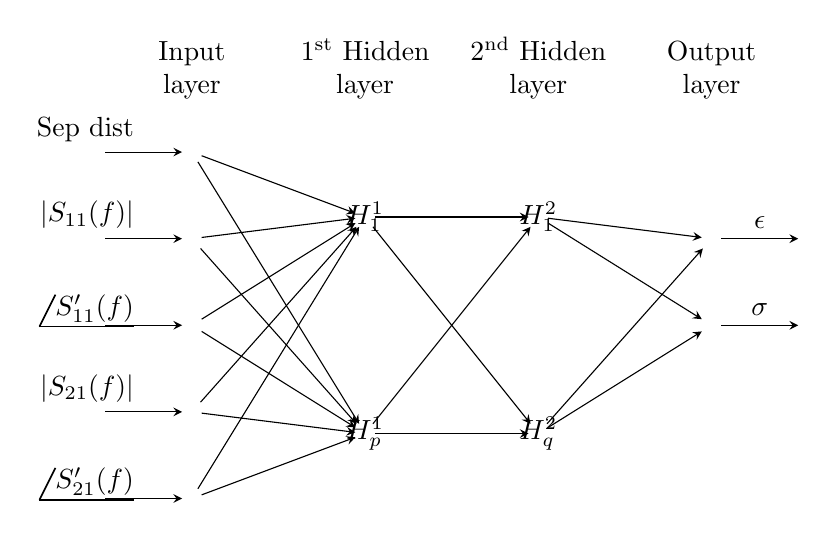
\begin{tikzpicture} [x=1.1cm, y=1.1cm, >=stealth]

\foreach \m/\l [count=\y] in {1}
  \node [every inputNeuron/.try, inputNeuron \m/.try] (input-\m) at (0,2.5-\y) {};

\foreach \m/\l [count=\y] in {2,3,4,5}
  \node [every multiNeuron/.try, multiNeuron \m/.try] (input-\m) at (0,2.5-\y-1) {};

\foreach \m [count=\y] in {1,missing,2}
  \node [every neuron/.try, neuron \m/.try ] (hidden-\m) at (2,2-\y*1.25) {};

\foreach \m [count=\y] in {1,missing,2}
	\node [every neuron/.try, neuron \m/.try ] (hiddenTwo-\m) at (4,2-\y*1.25) {};

\foreach \m [count=\y] in {1,2}
  \node [every neuron/.try, neuron \m/.try ] (output-\m) at (6,1.5-\y) {};

%\foreach \l [count=\i] in {1,2,3,n}
%  \draw [<-] (input-\i) -- ++(-1,0)
 %   node [above, midway] {$I_\l$};
    
\draw [<-] (input-1) -- ++(-1,0)
	node [above left, midway] {Sep dist};
	
\draw [<-] (input-2) -- ++(-1,0)
	node [above left, midway] {$|S_{11}(f)|$};
	
\draw [<-] (input-3) -- ++(-1,0)
	node [above left, midway] {$\phase{S_{11}'(f)}$};
	
\draw [<-] (input-4) -- ++(-1,0)
	node [above left, midway] {$|S_{21}(f)|$};
	
\draw [<-] (input-5) -- ++(-1,0)
	node [above left, midway] {$\phase{S_{21}'(f)}$};

\foreach \l [count=\i] in {1,p}
  \node at (hidden-\i) {$H^1_{\l}$};
  
\foreach \l [count=\i] in {1,q}
  \node at (hiddenTwo-\i) {$H^2_{\l}$};

\foreach \l [count=\i] in {\epsilon,\sigma}
  \draw [->] (output-\i) -- ++(1,0)
    node [above, midway] {$\l$};

\foreach \i in {1,...,5}
  \foreach \j in {1,...,2}
    \draw [->] (input-\i) -- (hidden-\j);
    
\foreach \i in {1,...,2}
  \foreach \j in {1,...,2}
    \draw [->] (hidden-\i) -- (hiddenTwo-\j);

\foreach \i in {1,...,2}
  \foreach \j in {1,...,2}
    \draw [->] (hiddenTwo-\i) -- (output-\j);

\foreach \l [count=\x from 0] in {Input, 1\textsuperscript{st} Hidden, 2\textsuperscript{nd} Hidden, Output}
  \node [align=center, above] at (\x*2,2) {\l \\ layer};

\label{fig:ANN}
\end{tikzpicture}


\newpage

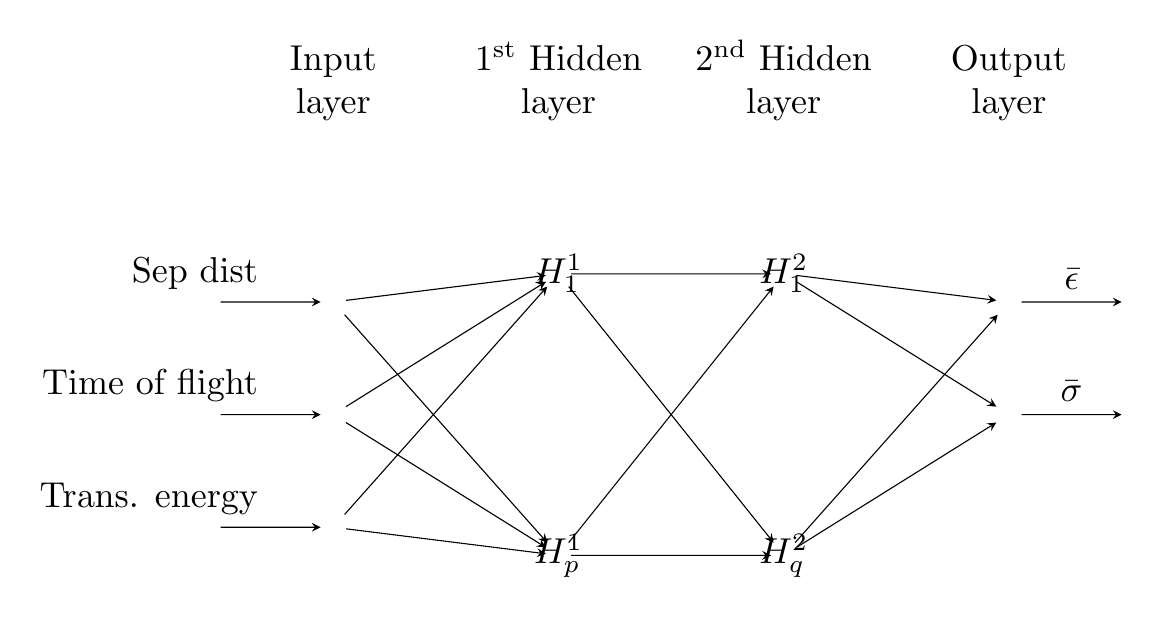
\begin{tikzpicture} [x=1.1cm, y=1.1cm, >=stealth, scale=1.3, every node/.style={scale=1.3}]

\foreach \m/\l [count=\y] in {1}
  \node [every inputNeuron/.try, inputNeuron \m/.try] (input-\m) at (0,2.5-\y-1) {};

%\foreach \m/\l [count=\y] in {2,3}
%  \node [every dualNeuron/.try, dualNeuron \m/.try] (input-\m) at (0,2.5-\y-2) {};
\foreach \m/\l [count=\y] in {2,3}
  \node [every splitNeuron/.try, splitNeuron \m/.try] (input-\m) at (0,2.5-\y-2) {\nodepart{second} \phantom{test}};

\foreach \m [count=\y] in {1,missing,2}
  \node [every neuron/.try, neuron \m/.try ] (hidden-\m) at (2,2-\y*1.25) {};

\foreach \m [count=\y] in {1,missing,2}
	\node [every neuron/.try, neuron \m/.try ] (hiddenTwo-\m) at (4,2-\y*1.25) {};

\foreach \m [count=\y] in {1,2}
  \node [every neuron/.try, neuron \m/.try ] (output-\m) at (6,1.5-\y) {};

%\foreach \l [count=\i] in {1,2,3,n}
%  \draw [<-] (input-\i) -- ++(-1,0)
 %   node [above, midway] {$I_\l$};
    
\draw [<-] (input-1) -- ++(-1,0)
	node [above left, midway] {Sep dist};
	
\draw [<-] (input-2) -- ++(-1,0)
	node [above left, midway] {Time of flight};
	
\draw [<-] (input-3) -- ++(-1,0)
	node [above left, midway] {Trans. energy};


\foreach \l [count=\i] in {1,p}
  \node at (hidden-\i) {$H^1_{\l}$};
  
\foreach \l [count=\i] in {1,q}
  \node at (hiddenTwo-\i) {$H^2_{\l}$};

\foreach \l [count=\i] in {\bar{\epsilon},\bar{\sigma}}
  \draw [->] (output-\i) -- ++(1,0)
    node [above, midway] {$\l$};

\foreach \i in {1,...,3}
  \foreach \j in {1,...,2}
    \draw [->] (input-\i) -- (hidden-\j);
    
\foreach \i in {1,...,2}
  \foreach \j in {1,...,2}
    \draw [->] (hidden-\i) -- (hiddenTwo-\j);

\foreach \i in {1,...,2}
  \foreach \j in {1,...,2}
    \draw [->] (hiddenTwo-\i) -- (output-\j);

\foreach \l [count=\x from 0] in {Input, 1\textsuperscript{st} Hidden, 2\textsuperscript{nd} Hidden, Output}
  \node [align=center, above] at (\x*2,2) {\l \\ layer};

\label{fig:ANN}
\end{tikzpicture}


\newpage

\tikzset{
    data/.style={
        draw,
        rectangle split,
        rectangle split parts=3,
        text centered,
    },
    data+/.style={
        data,
        rectangle split every empty part={},% resets empty-part macro (explanation below)
        rectangle split empty part width=\widthof{#1},
        rectangle split empty part height=\heightof{#1},
        rectangle split empty part depth=\depthof{#1},
    },
}
\newcommand{\data}{data \nodepart{second} \phantom{null}}

\tikzstyle{sim} = [rectangle, rounded corners, minimum width=3cm, minimum height=1cm,text centered, draw=black, fill=red!20]

\tikzstyle{prep} = [rectangle, rounded corners, minimum width=3cm, minimum height=1cm,text centered, draw=black, fill=blue!20]

\tikzstyle{ml} = [rectangle, rounded corners, minimum width=3cm, minimum height=1cm,text centered, draw=black, fill=gray!20]

\tikzstyle{mtos} = [rectangle, rounded corners, minimum width=3cm, minimum height=1cm,text centered, draw=black, fill=green!20]

\begin{tikzpicture}

\def\x{4.5}
\def\y{1.5}

% 
%  

\node (dat) {\begin{tabular}{c} \textbf{Data generation} \\ $ \mathcal{S}: [\vec{\epsilon}, \vec{\sigma}, \vec{d}]  \rightarrow \mathbf{X} \in \mathbb{C}^{n\times 4}$ \end{tabular}};
\node (pre) [right of = dat, node distance = \x cm] {\begin{tabular}{c} \textbf{Preprocessing} \\ $f: \mathbf{X} \rightarrow \vec{Y} \in \mathbb{R}^m$ \end{tabular}};
\node (mal) [right of = pre, node distance = \x cm] {\begin{tabular}{c} \textbf{Machine learning} \\ $g: [\vec{Y}, d] \rightarrow \vec{\mathcal{D}}_{bulk}$ \end{tabular}};

\node (simulation) [sim, below of = dat, node distance = \y cm] {\begin{tabular}{c} Homogeneous \\ \hline Layered \\ \hline  Realistic \end{tabular}};
\node (preproc) [prep, right of= simulation, node distance = \x cm] {\begin{tabular}{c} Peaks analysis \\ Energy analysis \\ Wavelet analysis \end{tabular}};
\node (ml) [ml, right of = preproc, node distance = \x cm] {\begin{tabular}{c} Neural networks \\ Elastic net \end{tabular} };

\draw[->,style=thick] (simulation) to (preproc);
\draw[->,style=thick] (preproc) to (ml);

\end{tikzpicture}



\newpage
\begin{tikzpicture}

\def\x{4.5}
\def\y{1.5}

\node (dat) {\begin{tabular}{c} \textbf{Measurement} \\ $ \mathbf{X}_{meas} \in \mathbb{C}^{n\times 4}$\end{tabular}};
\node (trans)  [right of = dat, node distance = \x cm] {\begin{tabular}{c} \textbf{Meas-sim conversion} \\ $ T: \mathbf{X}_{meas} \rightarrow \mathbf{X} $ \end{tabular}};
\node (pre) [right of = trans, node distance = \x cm] {\begin{tabular}{c} \textbf{Preprocessing} \\ $f: \mathbf{X} \rightarrow \vec{Y} \in \mathbb{R}^m$ \end{tabular}};
\node (mal) [right of = pre, node distance = \x cm] {\begin{tabular}{c} \textbf{Machine learning} \\ $g: [\vec{Y}, d] \rightarrow \vec{\mathcal{D}}_{bulk}$ \end{tabular}};


\node (simulation) [sim, below of = dat, node distance = \y cm] {\begin{tabular}{c} Measurement \\  of material \end{tabular}};
\node (meastosim) [mtos, right of = simulation, node distance = \x cm] {\begin{tabular}{c} Measurement \\ to simulation \\ transformation \end{tabular}};
\node (preproc) [prep, right of= meastosim, node distance = \x cm] {\begin{tabular}{c} Peaks analysis \\ Energy analysis \\ Wavelet analysis \end{tabular}};
\node (ml) [ml, right of = preproc, node distance = \x cm] {\begin{tabular}{c} Neural networks \\ Elastic net \end{tabular} };

\draw[->,style=thick] (simulation) to (meastosim);
\draw[->,style=thick] (meastosim) to (preproc);
\draw[->,style=thick] (preproc) to (ml);

\end{tikzpicture}



\newpage
\tikzstyle{line} = [draw, -latex']
\begin{tikzpicture}

\def\x{4}
\def\y{1.5}

\node (dat) {\begin{tabular}{c} \textbf{Data generation} \\ $ \mathcal{S}: [\vec{\epsilon}, \vec{\sigma}, \vec{d}]  \rightarrow \mathbf{X} \in \mathbb{C}^{2\times 2\times n}$\end{tabular}};
\node (pre) [right of = dat, node distance = \x cm] {\begin{tabular}{c} \textbf{Preprocessing} \\ $f: \mathbf{X} \rightarrow \vec{Y} \in \mathbb{R}^m$ \end{tabular}};
\node (mal) [right of = pre, node distance = \x cm] {\begin{tabular}{c} \textbf{Machine learning} \\ $g: [\vec{Y}, d] \rightarrow \vec{\mathcal{D}}_{bulk}$ \end{tabular}};

\node (simulation) [sim, below of = dat, node distance = \y cm] {\begin{tabular}{c} Homogeneous \\ \hline Layered \\ \hline  Realistic \end{tabular}};
\node (meastosim) [mtos, below right of =simulation, node distance = 2.5 cm] {\begin{tabular}{c} Meas $\rightarrow$ sim \end{tabular}};
\node (preproc) [prep, right of= simulation, node distance = \x cm] {\begin{tabular}{c} Peaks analysis \\ Energy analysis \\ Wavelet analysis \end{tabular}};
\node (ml) [ml, right of = preproc, node distance = \x cm] {\begin{tabular}{c} Neural networks \\ Elastic net \end{tabular} };

\node (trans)  [below of = meastosim, node distance = 1 cm] {\begin{tabular}{c} Measured? \\ $ T: \mathbf{X}_{meas} \rightarrow \mathbf{X} $ \end{tabular}};

\node (output) [right of = ml, node distance = \x cm] {$\mathcal{D}_{bulk}$};
\node (input) [left of = simulation, node distance = \x cm] {\begin{tabular}{c} Training? \\ $ [\vec{\epsilon}, \vec{\sigma}, \vec{d}]$\end{tabular}};
\node [below right of = ml, node distance = 1.5 cm] {$\mathcal{D}_{bulk_true}$};

\draw[->,style=thick] (simulation) -- (preproc);
\draw[->,style=thick] (input) -- (simulation);
\draw[->,style=thick] (simulation) to (meastosim);
\draw[->,style=thick] (meastosim) to (preproc);
\draw[->,style=thick] (preproc) to (ml);
\draw[->,style=thick] (ml) to (output);
%\draw[->, style=thick] (input) to (ml);
%\path[line] (input) |- ([xshift=-0.5cm,yshift=-3.5cm]simulation.south west) |- (ml);
\draw[->] (input) to ([xshift=-2.5cm,yshift=-3.3cm]simulation.south west) to  ([xshift=1.5cm,yshift=-3.5cm]ml.south west) to (ml);

\end{tikzpicture}


% multidimensional plots
% homogeneous
\newpage

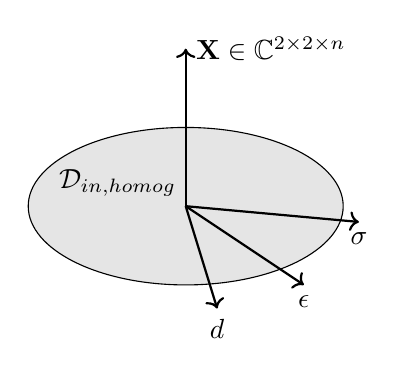
\begin{tikzpicture}

\draw [fill=gray!20] (0,0) ellipse (2cm and 1cm) node[above left] {$\mathcal{D}_{in, homog}$};


\draw[->, thick] (0,0) to (0.4,-1.3) node[below] {$d$};
\draw[->, thick] (0,0) to (1.5,-1) node[below] {$\epsilon$};
\draw[->, thick] (0,0) to (2.2,-0.2) node[below] {$\sigma$};



\draw[->, thick] (0,0) to (0,2) node[right] {$\mathbf{X} \in \mathbb{C}^{2\times 2 \times n}$};

\end{tikzpicture}


% layered
\newpage

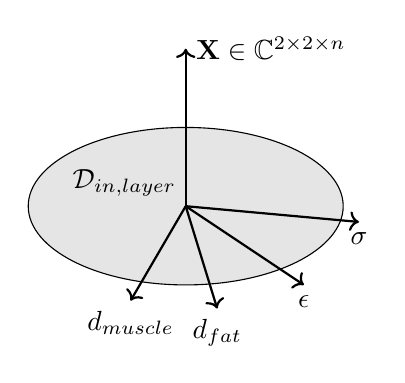
\begin{tikzpicture}

\draw [fill=gray!20] (0,0) ellipse (2cm and 1cm) node[above left] {$\mathcal{D}_{in, layer}$};


\draw[->, thick] (0,0) to (-0.7,-1.2) node[below] {$d_{muscle}$};
\draw[->, thick] (0,0) to (0.4,-1.3) node[below] {$d_{fat}$};
\draw[->, thick] (0,0) to (1.5,-1) node[below] {$\epsilon$};
\draw[->, thick] (0,0) to (2.2,-0.2) node[below] {$\sigma$};



\draw[->, thick] (0,0) to (0,2) node[right] {$\mathbf{X} \in \mathbb{C}^{2\times 2 \times n}$};

\end{tikzpicture}



% realistic
\newpage

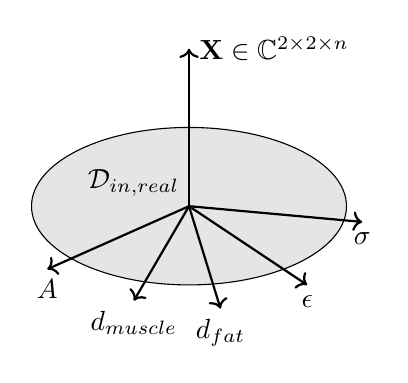
\begin{tikzpicture}

\draw [fill=gray!20] (0,0) ellipse (2cm and 1cm) node[above left] {$\mathcal{D}_{in,real}$};

\draw[->, thick] (0,0) to (-1.8,-0.8) node[below] {$A$};
\draw[->, thick] (0,0) to (-0.7,-1.2) node[below] {$d_{muscle}$};
\draw[->, thick] (0,0) to (0.4,-1.3) node[below] {$d_{fat}$};
\draw[->, thick] (0,0) to (1.5,-1) node[below] {$\epsilon$};
\draw[->, thick] (0,0) to (2.2,-0.2) node[below] {$\sigma$};



\draw[->, thick] (0,0) to (0,2) node[right] {$\mathbf{X} \in \mathbb{C}^{2\times 2 \times n}$};

\end{tikzpicture}


% neuron figures
\newpage

\tikzstyle{neuron} = [circle split, minimum size=0.8cm,text centered, text=white, draw=white, fill=gray]
\tikzstyle{neuronNoSplit} = [circle, minimum size=0.8cm,text centered, text=white, draw=white, fill=gray]
\tikzstyle{io} = [circle, rounded corners, minimum size=0.8cm, text centered, draw=gray, fill=white!30]
\tikzstyle{outs} = [rectangle, rounded corners, minimum size=0.8cm, text centered, draw=white, fill=white!30]
\tikzstyle{arrow} = [thick,->,>=stealth]

\centering
\begin{tikzpicture}[node distance = 2cm]
\node (outputs) [outs] {Outputs:};
\node (outs) [outs, below = 0.2 cm of outputs] {$\chi(\textbf{w}^t \cdot \textbf{x} + \theta)$};
\node (neuron) [neuron, below of = outs] {$\chi ( )$ \nodepart{lower} $\sum$};
\node (w2) [io, below = 0.6cm of neuron] {$w_2$};
\node (w1) [io, below left = 0.7cm and 0.1cm of neuron] {$w_1$};
\node (w3) [io, below right = 0.7cm and 0.1cm of neuron] {$w_3$};
\node (io2) [outs, below = 0.6cm of w2] {$x_2$};
\node (io1) [outs, below left = 0.7cm and 0.1cm of w1] {$x_1$};
\node (io3) [outs, below right = 0.7cm and 0.1cm of w3] {$x_3$};
\node (bias) [io, left of = neuron] {$\theta$};
%\node[circle split] {$\sigma$ \nodepart{lower}$\sum$};

\draw [arrow] (w1) -- (neuron);
\draw [arrow] (w2) -- (neuron);
\draw [arrow] (w3) -- (neuron);
\draw [arrow] (neuron) -- (outs);
\draw [arrow] (bias) -- (neuron);

\draw[thick] (io1) -- (w1);
\draw[thick] (io2) -- (w2);
\draw[thick] (io3) -- (w3);

\end{tikzpicture}



% gradient descent
\newpage
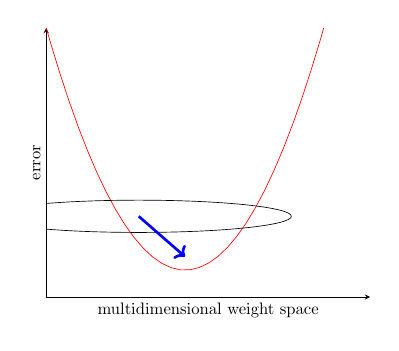
\begin{tikzpicture}[scale = 0.6]
\begin{axis}[
	ticks=none,
    axis lines = left,
    %xlabel = $x$,
    ylabel = {error},
    xlabel = {multidimensional weight space},
    ymin = 2, ymax = 12,
    xmin = -2, xmax = 5
]
%Below the red parabola is defined
\addplot [
    domain=-10:10, 
    samples=100, 
    color=red,
]
{x^2 - 2*x + 4};

\draw (axis cs:0,5) ellipse [x radius = 3.3, y radius = 0.6, fill=blue,];

\draw[->,blue,ultra thick] (axis cs:0,5) to (axis cs:1,3.5);
 
\end{axis}

\end{tikzpicture}


\end{document}